\documentclass{scrreprt}
\usepackage[english]{babel}
\usepackage[T1]{fontenc}
\usepackage{lmodern}
\usepackage{blindtext}
\usepackage[utf8]{inputenc}
\usepackage{siunitx} %For unit handling%
\renewcommand{\familydefault}{\sfdefault}
\newcommand{\unit}[1]{\ensuremath{\, \mathrm{#1}}}
\usepackage{amssymb, amsmath, cancel, ulem, graphicx, float, tabularx, multirow, bm}
\usepackage{amsmath}
\usepackage{caption}
\usepackage{subcaption}
\usepackage{mathtools}
\usepackage{tikz}
\newcommand*\circled[1]{\tikz[baseline=(char.base)]{
            \node[shape=circle,draw,inner sep=1pt] (char) {#1};}}
\renewcommand{\phi}{\varphi}


\setcounter{secnumdepth}{5}
\setcounter{tocdepth}{5}

\author{Urs Gerber\\09-921-156 \and Gian-Luca Mateo\\11-113-545}
\date{18th of April 2013}

\title{Coupled pendulums}
\subtitle{Practical course report}

\begin{document}

\maketitle

\tableofcontents
\newpage

\chapter{Experiment: Coupled pendulums}

\section{Introduction}

\subsection{Goal of the experiment}

\subsection{Theory}

\subsection{Uncertainty analysis}

\section{Experiment setup and execution}

\subsection{Used materials}
The materials used in this experiment are the following:
\begin{itemize}
\item An assembly (labelled No.$3$) with two ball bearing mounted sticks ($21.37\unit{g}$ each), which have threaded bottoms
\item Two weights ($214.15 \unit{g}$ each) with threaded holes which can be screwed onto the bottom of the sticks and secured with two nuts ($2\unit{g}$ each)
\item two brackets, mountable to the sticks
\item a spring, attachable to the brackets 
\item a ruler, metric scale, $38 \unit{cm}$ long
\item a mechanical stopwatch, $0.2 \unit{s}$ steps
\end{itemize}

\subsection{Assembly}
For our measurements, the materials are assembled as shown in image \ref{fig:assembly}.

\begin{figure}[H]
	\centering
  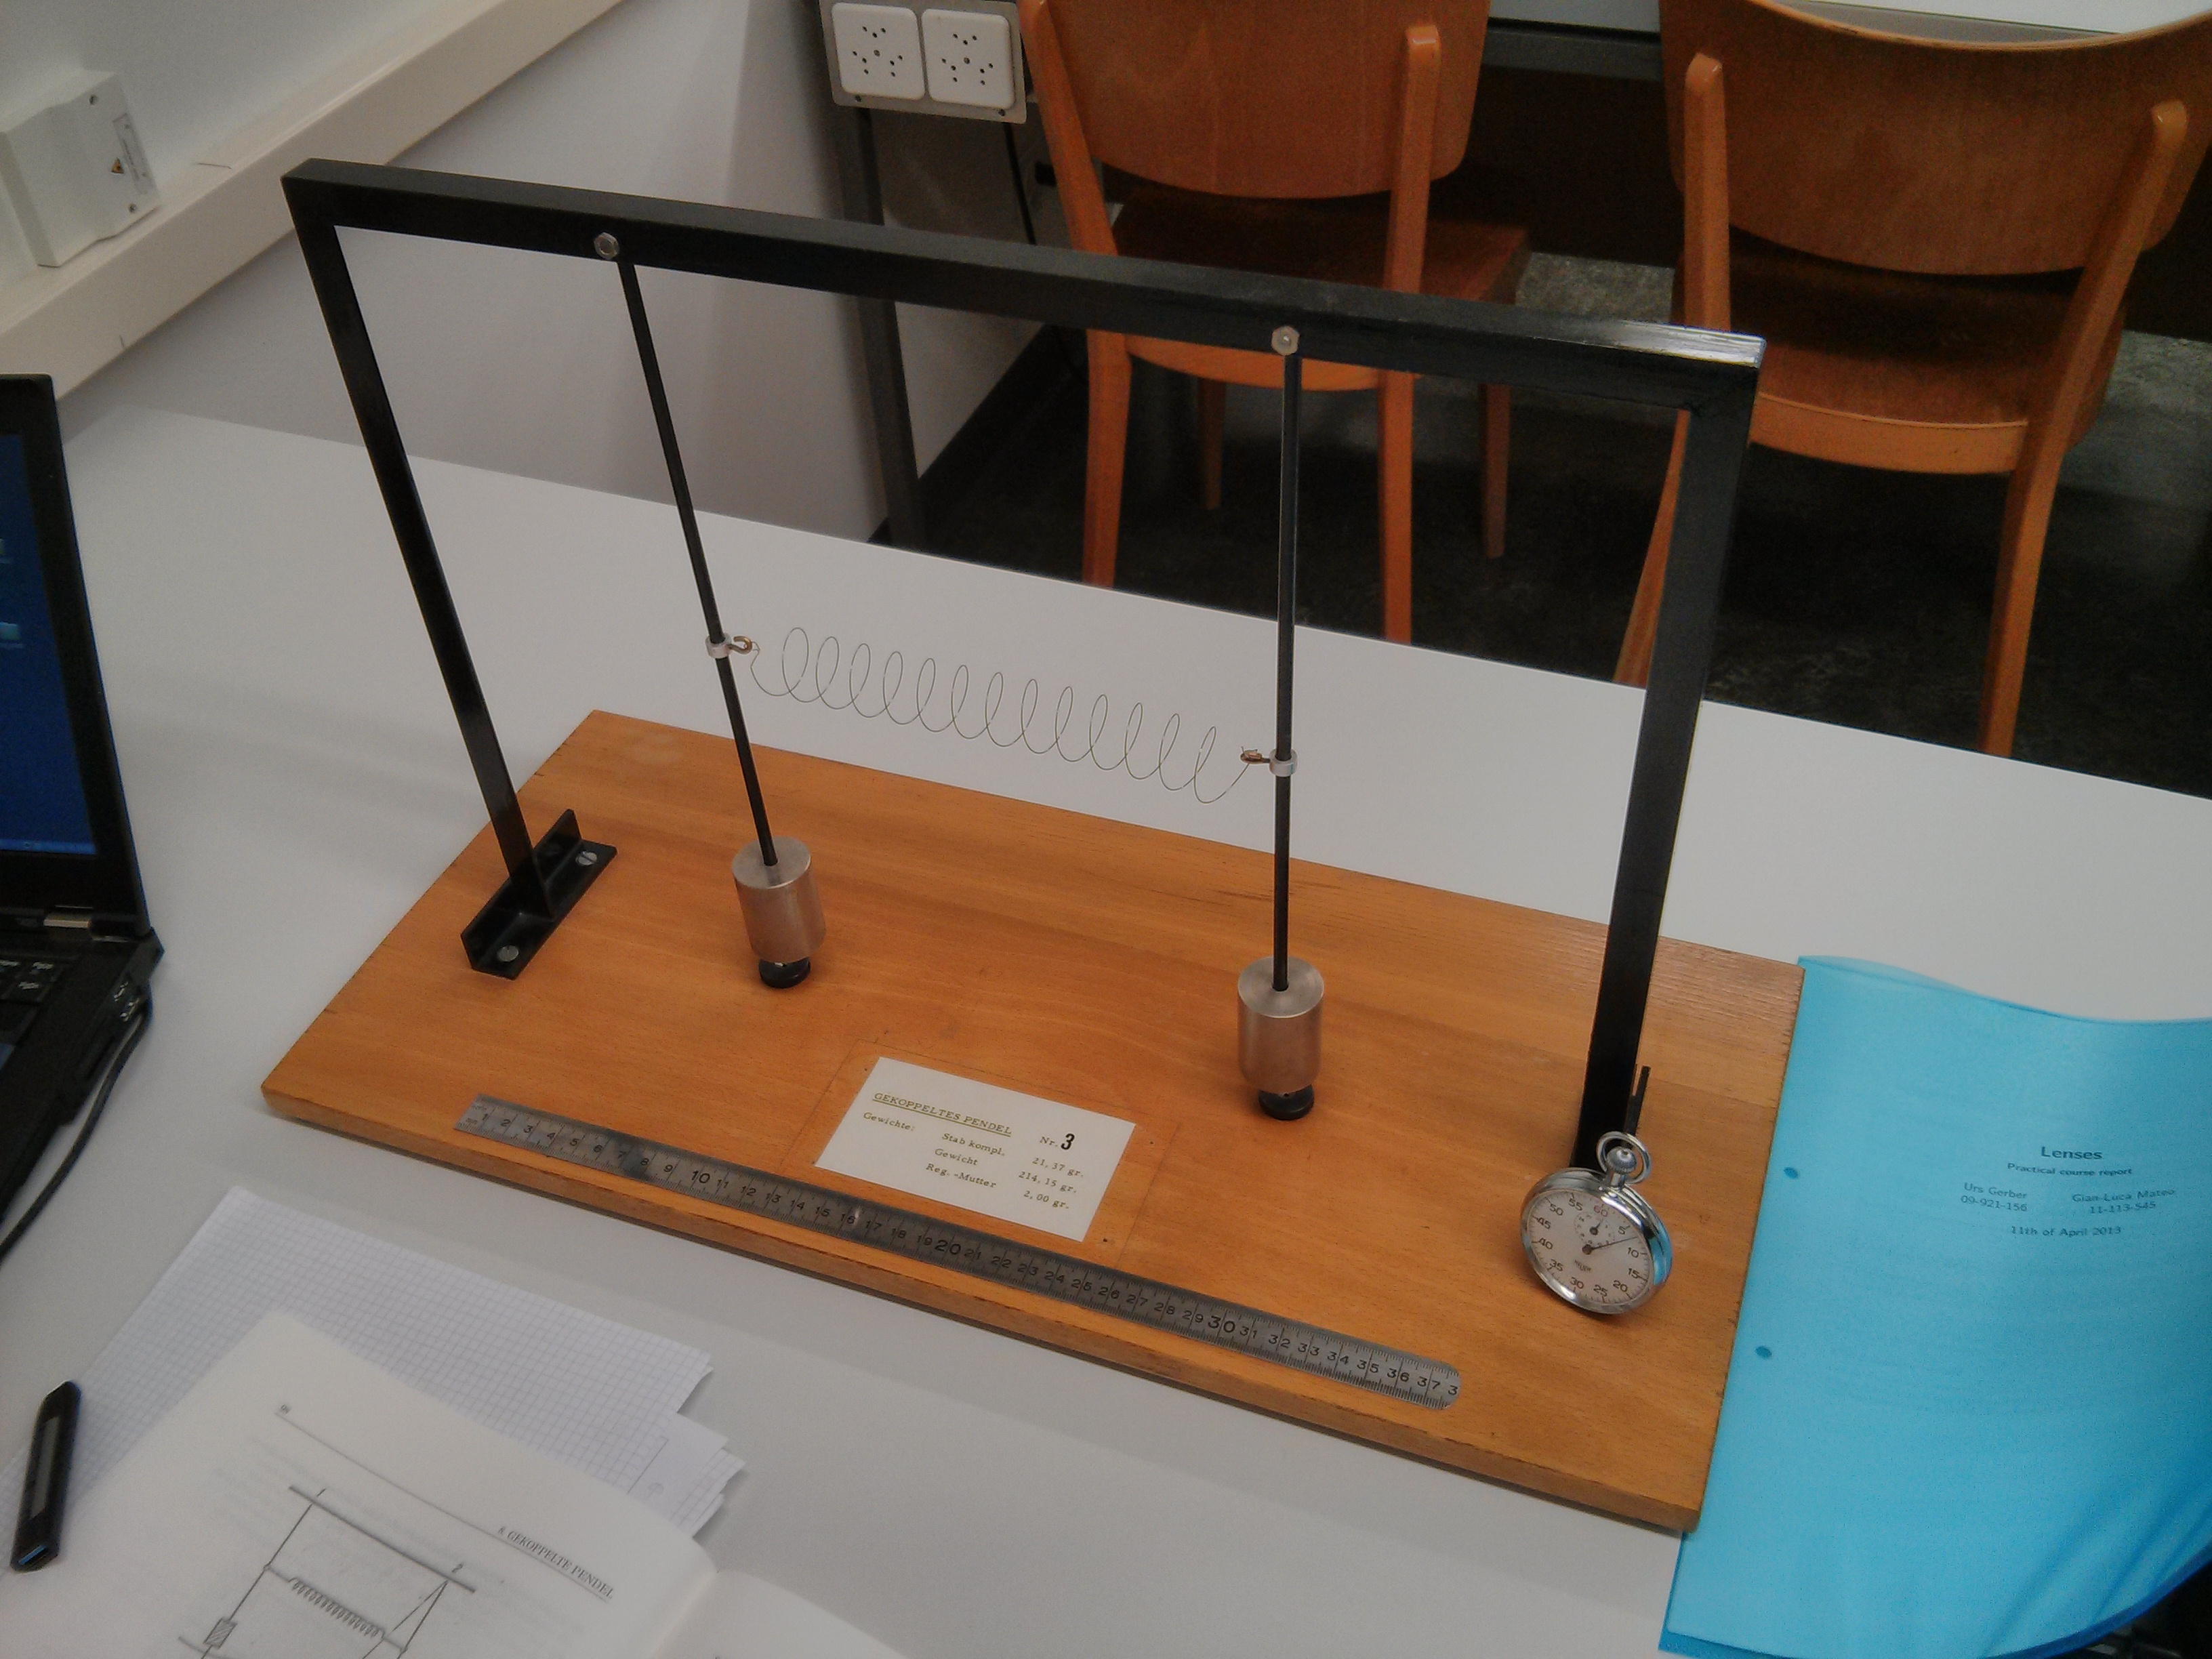
\includegraphics[width=0.9\textwidth]{img/assembly.jpg}
	\caption{Experiment Assembly}
	\label{fig:assembly}
\end{figure}
For the first series of measurements, one pendulum is detached from the spring, deflected and its oscillation period measured. for the second series, the weight at the bottom of the second pendulum is moved up or down in order to obtain the same period as the first one. Next, the spring is attached to both pendulums at the same height. Once this is done, the following values are measured:
\begin{itemize}
\item $\tau_{\omega}$: in-phase oscillation period, $\phi_1 = \phi_2$
\item $\tau_{\Omega}$: opposite in-phase oscillation period, $\phi_1 = -\phi_2$
\item $\tau$ : paraphase oscillation period, $\phi_1 = 0, \phi_2 = \Phi$
\item $T_s$ : beat period
\end{itemize}
\section{Measurements}

\section{Analysis and Discussion}

\section{Conclusion}

\begin{thebibliography}{9}

\bibitem{physcript13}
  Peter Wurz,
  \emph{Anleitung zum Physikpraktikum}
  FS2013

\end{thebibliography}

\end{document}
